\section*{Procedimiento Laboratorio}

\section{Alineación del sistema}
Familiarizarse con el montaje hecho para este
experimento, mostrado en la Figura 1.

\begin{figure}[H]
    \centering
    \begin{subfigure}[b]{0.45\textwidth}
        \centering
        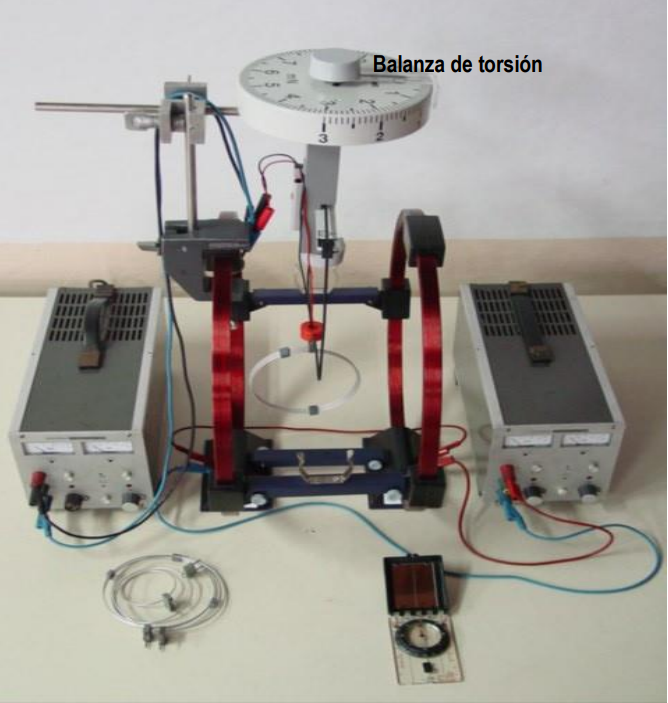
\includegraphics[width=\textwidth]{Figures/0. General/1.1.png}
        \caption{\textit{Figura 1. Montaje para la medida del torque producido en una espira.}}
        \label{Figura 1}
    \end{subfigure}
\end{figure}

Se realizó el siguiente montaje, con dos fuentes de alimentación de energía, la
primera lleva corriente a las bobinas de Helmholtz creando un campo magnético
constante, la segunda lleva corriente a la espira, cuyo vector de área debe ser
perpendicular a la dirección del campo magnético, la corriente en movimiento
alrededor de la espira circular, genera un campo magnético que interactúa con
el campo de las bobinas, provocando un torque o movimiento de la espira, la
fuerza de dicho torque se calcula experimentalmente con el dinamo de torsión,
este al estar conectado a la espira se gira para llevarla a su posición
original y nos muestra la fuerza necesaria para esta acción, la cual es
equivalente a la fuerza del torque que la desacomodó de su posición inicial.
Ahora bien, el montaje fue de la siguiente manera:

\begin{figure}[H]
    \centering
    \begin{subfigure}[b]{0.45\textwidth}
        \centering
        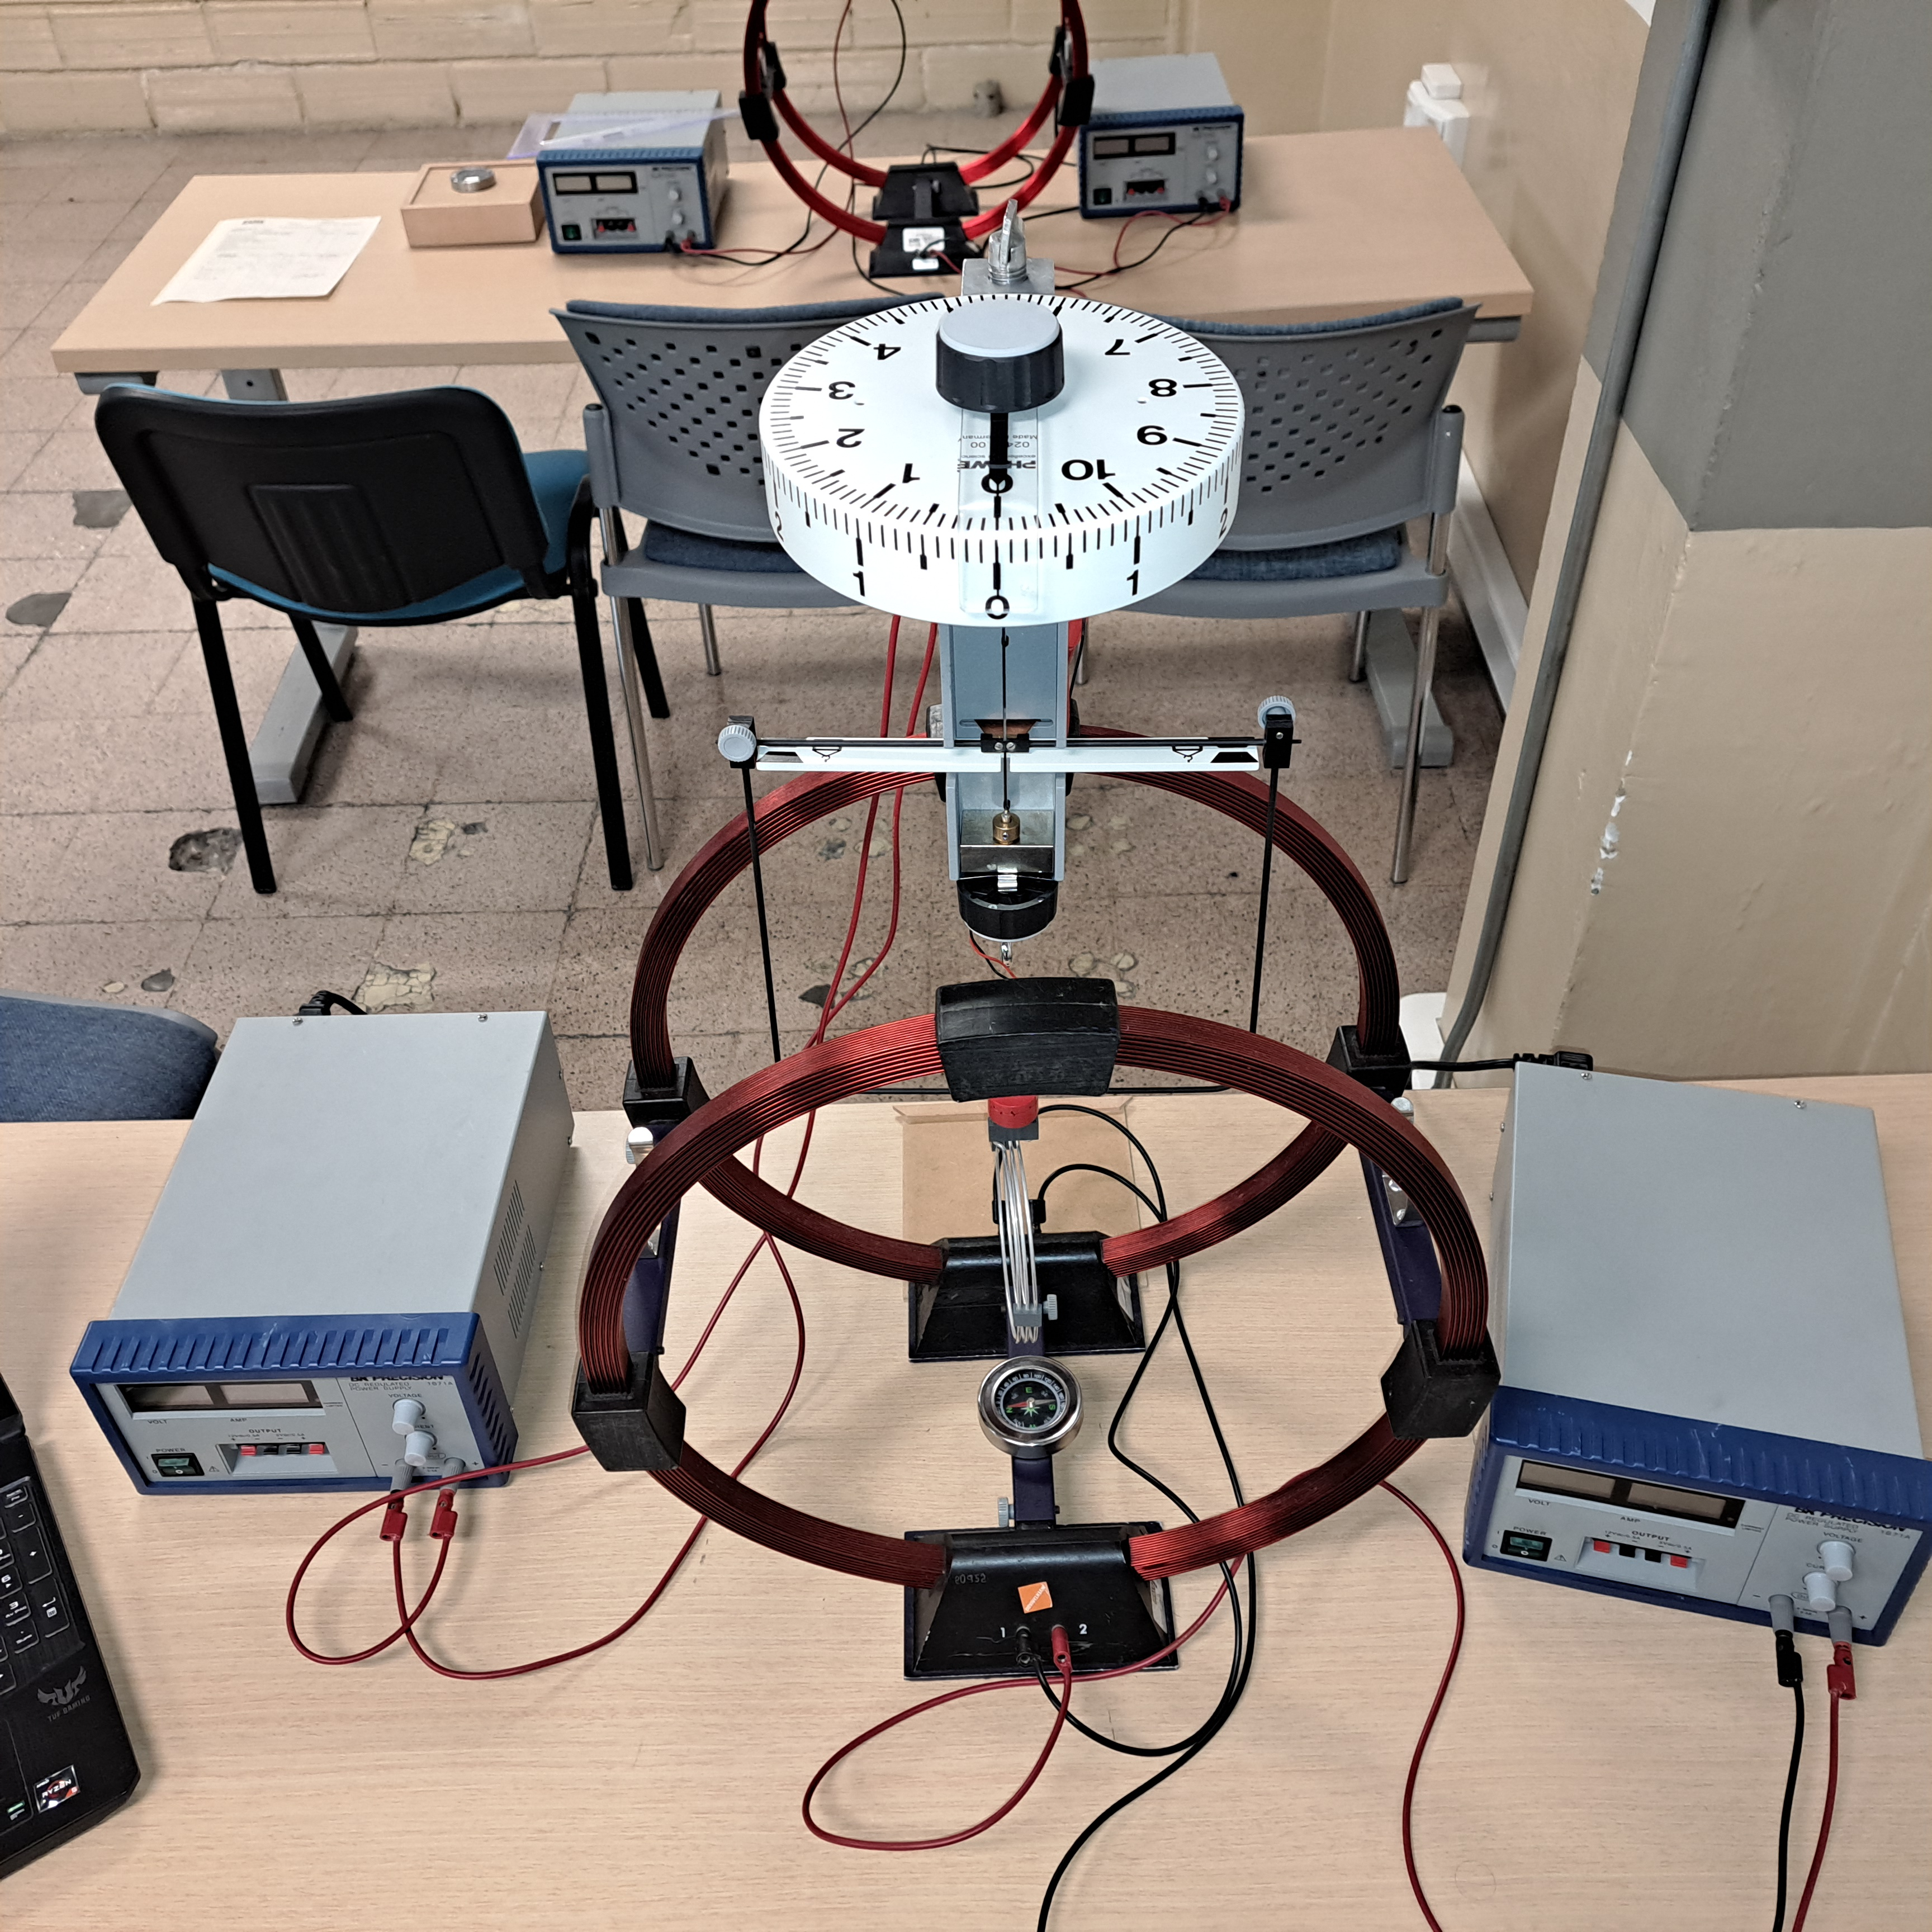
\includegraphics[width=\textwidth]{Figures/0. General/1.2.jpg}
        \caption{\textit{Figura 2. Montaje propio para la medida del torque producido en una espira.}}
        \label{Figura 2}
    \end{subfigure}
\end{figure}

\section{Calcular intensidad del Campo Magnético}

Ajustar la corriente $I$ (de las bobinas de Helmholtz) a $3A$ . Con ayuda de una
brújula notar la presencia de un campo magnético en el interior de la bobina.
Con los parámetros fijados y con la expresión de Helmholtz, calcular la
intensidad del campo magnético.
\\
\textit{Expresión de Helmholtz:}

\[B = \mu_0 \times 0.715 \times M \times \frac{I}{R} \]


\begin{figure}[H]
    \centering
    \begin{subfigure}[b]{0.5\textwidth}
        \centering
        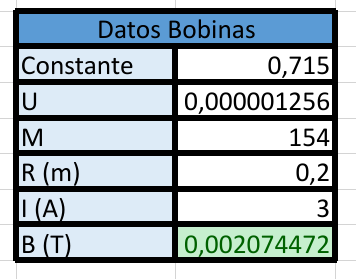
\includegraphics[width=\textwidth]{Figures/0. General/2.1.png}
        \caption{\textit{Figura 3. Calculo de intensidad del Campo Magnético}}
        \label{Figura 3}
    \end{subfigure}
\end{figure}


\section{Cálculo de Torque con bobina 1}

Apagar las fuentes y colocar en la balanza de torsión una bobina de prueba de
$N_3 = 3$ espiras, de tal forma tal que el ángulo entre el campo magnético y la
normal a la bobina de prueba sea $\theta = 90^{\circ}$. Con las dos fuentes
apagadas, ajustar la posición de la balanza de torsión en cero

\subsection{Encender y ajustar las fuentes}

Encender y ajustar las fuentes para que circule una corriente $i = 0.5A$ por la
bobina de prueba de tres vueltas y establecer $I = 3A$ por las bobinas de
Helmohltz. El montaje fue el siguiente:
\dots

\subsection{Medir desplazamiento}

Volver a equilibrar la balanza y medir este desplazamiento; esto es, la fuerza
aplicada en el brazo del dinamómetro $\tau_{E} = F \times d$, donde $d = 0.11m$
y $F$ es la lectura del dinamómetro (en milinewtons).

\subsection{Repetir}

Repetir los pasos anteriores con las corrientes que se muestran en la
tabla siguiente:

\subsection{Graficar $\tau_{T}$ vs $i$}

Graficar $\tau_{T}$ vs $i$, teórico y práctico en un mismo plano cartesiano y
encontrar la pendiente. Además, describir el significado físico de esta
pendiente.


\section{Cálculo de Torque Torque con bobina 2}

Utilizar los siguientes parámetros: $i = 3A$, $N_3 = 3$, $\theta = 90^{\circ}$.
Apagar las fuentes y ajustar la balanza a su posición de cero.

\subsection{Variar la corriente \textit{I}}

Variar la corriente \textit{I} de acuerdo a los valores de la siguiente tabla:


\subsection{Calcular el campo magnético \textit{B}}

Calcular el campo magnético \textit{B} con cada valor de corriente y graficar
$\theta$ vs $B$, tanto teórica como experimentalmente en un mismo
plano cartesiano y encontrar la pendiente. Además, identificar el
significado físico de esta pendiente.


\section{Cálculo de Torque Torque por cantidad de espiras}

Ajustar $I = i = 3A$ y $\theta = 90^{\circ}$. Apagar las fuentes y conectar
bobinas de prueba de $3, 2, 1$ espiras de igual área y en cada caso hacer
medidas de torque.

\textit{Nota:} Al colocar cada espira con las fuentes apagadas se debe ajustar
la balanza en la posición de cero.

\subsection{Graficar $\tau$ vs $N$}

Graficar $\tau$ vs $N$, teórico y práctico en un mismo plano cartesiano,
obtener la pendiente y especificar su significado físico.

\section{Cálculo de Torque Torque por cantidad área de espiras}

Similar al literal anterior, conectar bobinas de 1 espira y diferente área, en
cada caso calcular el área y medir el torque. Ajustar $I = i = 3A$, $N = 1$ y
$\theta = 90^{\circ}$.


\subsection{Graficar $\tau$ vs $A$}

Graficar $\tau$ vs $A$, teórico y práctico en un mismo plano cartesiano,
obtener la pendiente y especificar su significado físico.


\section{Agregar en su informe comentarios, sugerencias, causas de error y
  conclusiones}

\subsection{Qué factores pueden afectar el cálculo experimental?}

\begin{itemize}
    \item En la toma de datos puede haber discrepancias:
          \subitem Esto se da por que puede llegar a existir un error en la
          calibración del equipo.
          \subitem Esto se da por que puede llegar a existir un error en la
          a la hora de medir algunos valores.
\end{itemize}


\subsection{Conclusiones}

En este informe número 6, pudimos ver:

\begin{itemize}
    \item Se logra medir el torque magnético y se demostró las relaciones que
          tienen cada una de las cantidades con el torque, y de este modo
          desarrollando una mayor comprensión de la teoría abordada.
    \item Identificamos la presencia de campos magnéticos con ayuda de una
          brújula, debido a que la aguja se alineó en la dirección de dichos
          campos, permitiendonos una "imagen más o menos mental" de estos campos.
\end{itemize}



\subsection{Imanes}

\subsubsection{Determine las líneas de campo de los diferentes imanes}
Con las limaduras de hierro determine las líneas de campo de los diferentes
imanes, como se muestra en la figura adjunta.


\subsubsection{Encontrar los polos norte y sur}
Con dos imanes encontrar los polos norte y sur de cada uno de ellos.


\subsubsection{Para dos imanes comprobar}
Para dos imanes comprobar que polos magnéticos del mismo tipo se repelen y polos
magnéticos de distinto tipo se atraen.

Se trata de manejar una pareja de imanes y observar las posiciones en donde la
atracción es máxima y las posiciones en donde la repulsión es máxima.
Igualmente, se trata de visualizar el campo magnético con limaduras de hierro en
las siguientes situaciones:

\begin{itemize}
    \item Un imán.
    \item Dos imanes con polos idénticos enfrentados.
    \item Dos imanes con polos opuestos enfrentados.
\end{itemize}


\subsubsection{Teslámetro}
Con ayuda del teslámetro mida el campo magnético para una distancia constante en
diferentes imanes y determine cual tiene mayor fuerza magnética.


\subsubsection{Geometría del teslámetro}
De acuerdo con la geometría del teslámetro construya la siguiente tabla,
midiendo el campo magnético de tres imanes diferentes a diferentes distancias.

\begin{figure}[H]
    \centering
    \begin{subfigure}[b]{0.8\textwidth}
        \centering
        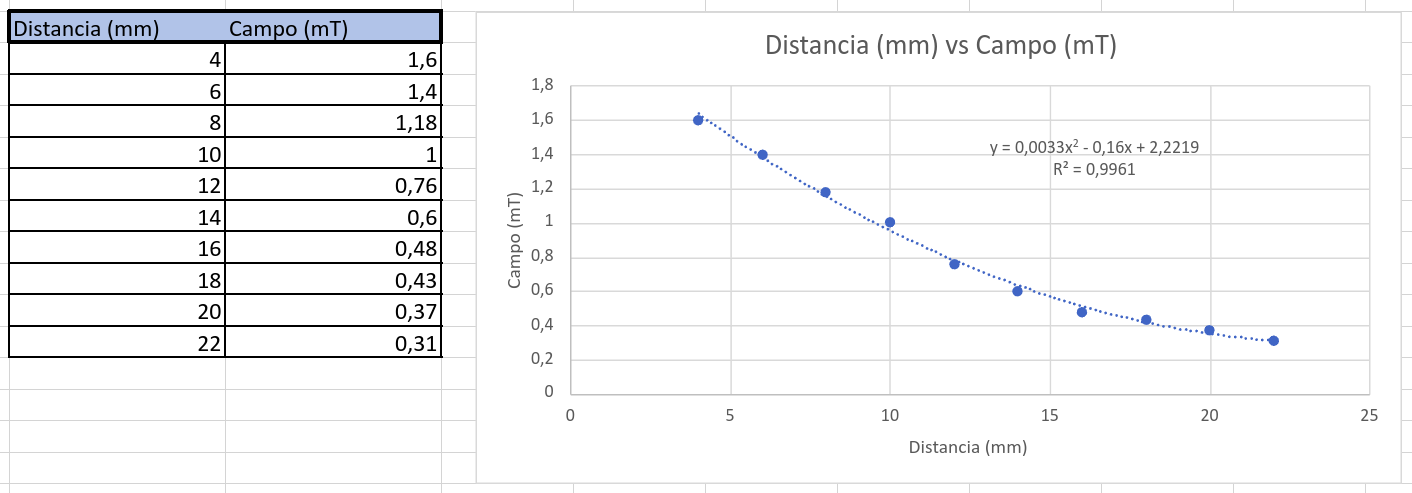
\includegraphics[width=\textwidth]{Figures/0. General/1.5.png}
        \caption{\textit{B vs d}}
        \label{fig: style 1 B vs d}
    \end{subfigure}
\end{figure}


\subsubsection{¿Cómo varía \textit{B} con \textit{d}?}
Analizando los resultados de la tabla y el grafico \textit{B vs d} que estos
resultados nos brindan, se comprueba que la medida del campo magnético depende
indirectamente de la distancia a la cual este se está midiendo, dado que este se
hace menor a medida que aumenta la distancia, y aumenta al reducir la distancia
del imán que lo genera con el teslámetro que lo mide.


\subsubsection{¿Qué significado tiene la expresión de que un imán es muy potente?}
Esta expresión hace referencia a su densidad de líneas de campo magnético,
porque al ser mayor, la fuerza magnética con la que atrae a otros imanes, o
algunos materiales metalicosmetálicos será mayor.


\subsubsection{Comparado con el campo magnético de la Tierra}
Comparado con el campo magnético de la Tierra, ¿qué orden de magnitud tienen los
valores que usted midió para el campo magnético de los imanes?\\

La tierra funciona como un gran imán cuya magnitud oscila entre:\\

\(2.5\times10^{-5}\) y \(6.5\times10^{-5}\) (T) Teslas siendo mayor en los polos
y menor cerca de la line del ecuador. Para la respuesta tendremos en cuenta que
la magnitud del campo magnético de la tierra medido en la superficie de la
tierra puede alcanzar un valor máximo de \(6.5\times10^{-5}\) (T) y que el
valor de campo magnético más grande alcanzado por uno de los imanes en el
laboratorio fue de \(4.02\times10^{-2}\).\\

Al analizar esto, se puede observar que el campo magnético de los imanes tiene
un orden de \(10^{-2}\) el cual es mil veces mayor ok que el de la tierra
que tiene un orden de magnitud de \(10^{-5}\).


\subsection{Campo magnético terrestre}

\subsubsection{Montaje Figura 2}
Realice el montaje mostrado en la Figura 2.


\subsubsection{brújula en el centro}
Sin haber encendido la fuente, coloque la brújula en el centro de las bobinas.
La dirección hacia donde apunta la brújula, es la dirección del campo magnético
terrestre. Ubique las bobinas de modo que su plano esté en la dirección delcampo
magnético terrestre, o sea que su eje este en la dirección este-oeste, como se
observa en la Figura 2.


\subsubsection{Encontrar los polos norte y sur}
Encienda la fuente de voltaje y ajuste una corriente hasta que la aguja de la
brújula se ubique en \(\phi = 10^\circ\). La aguja de la brújula se orienta en dirección del campo
magnético resultante de combinar el campo magnético de las bobinas y el campo
magnético terrestre. Tome la dirección norte-sur para medir los ángulos, es
decir, tome como la orientación de la aguja de la brújula cuando la corriente
por las bobinas es cero, como se observa en la Figura 2. Registre la medida de
la corriente mostrada en el miliamperímetro, en la casilla de la tabla que
aparece a continuación y calcule \textit{BH} con la relación (6): Sí no es posible colocar
la aguja de la brújula en los ángulos sugeridos, defina usted por lo menos 7
posiciones angulares y realice:


\begin{figure}[H]
    \centering
    \begin{subfigure}[b]{\textwidth}
        \centering
        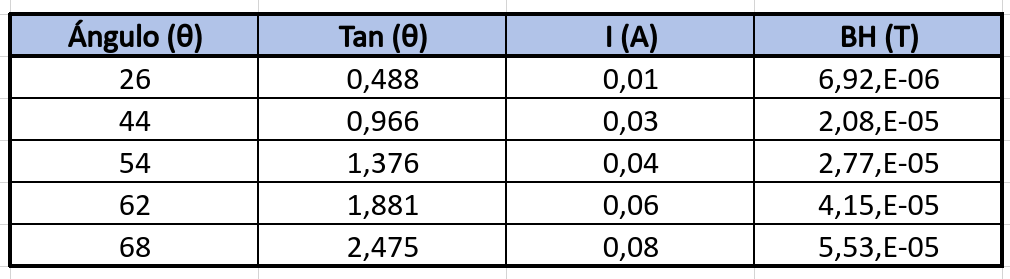
\includegraphics[width=\textwidth]{Figures/0. General/2.3.1.png}
        \caption{\textit{Tabla 1.2.3.1}}
    \end{subfigure}
\end{figure}

\begin{figure}[H]
    \centering
    \begin{subfigure}[b]{0.6\textwidth}
        \centering
        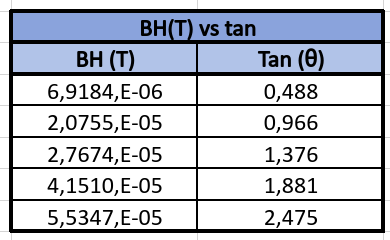
\includegraphics[width=\textwidth]{Figures/0. General/2.3.2.png}
        \caption{\textit{Tabla 1.2.3.2}}
    \end{subfigure}
\end{figure}



\subsubsection{Grafique \textit{BH(I)} vs \textit{tan\((\phi)\)}}
Grafique \textit{BH(I)} vs \textit{tan\((\phi)\)}:

\begin{figure}[H]
    \centering
    \begin{subfigure}[b]{\textwidth}
        \centering
        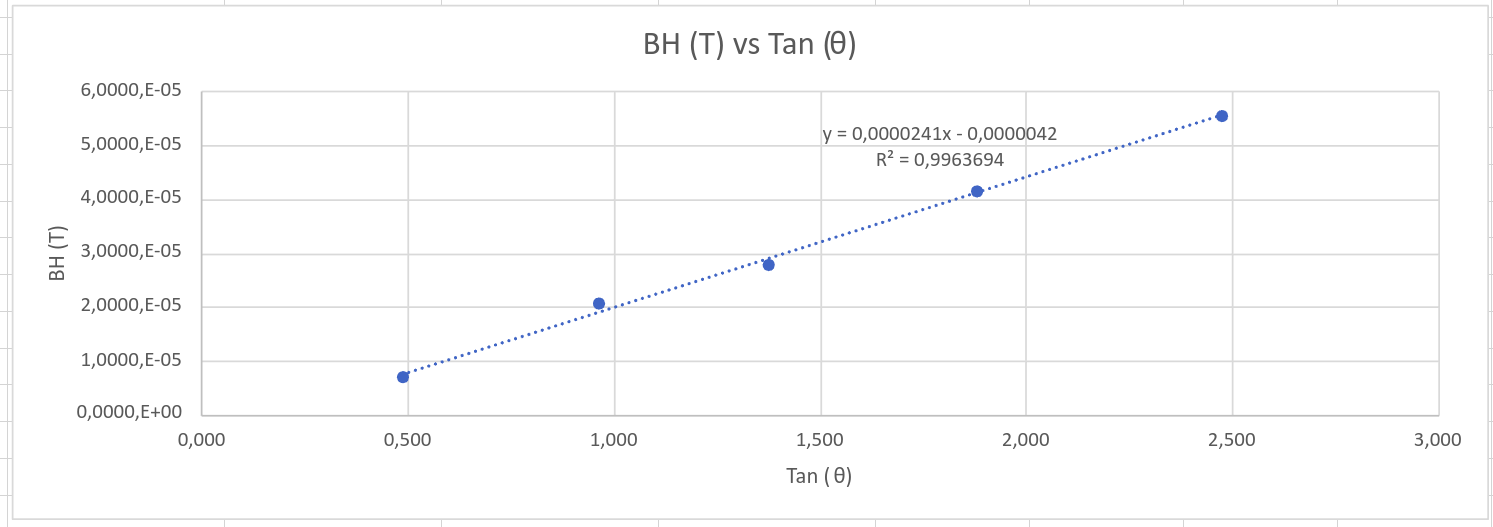
\includegraphics[width=\textwidth]{Figures/0. General/2.4.png}
        \caption{\textit{BH(I)} vs \textit{tan\((\phi)\)}}
    \end{subfigure}
\end{figure}


\subsubsection{campo magnético terrestre}
Encuentre el campo magnético terrestre haciendo uso de la pendiente de la
gráfica anterior (use regresión lineal).\\

Teniendo en cuenta la fórmula de la recta:
\[ y = mx\]

Y teniendo en cuenta la ecuación 7 de la orientación del ángulo de la brújula
sometida a ambos campos:

\[ Tan_{(\phi)} = \frac{B_{H}(I)}{B_{T}} \]

Despejemos $B_{H}$

\[ B_{H}(I) = Tan_{(\phi)} \times B_{T} \]

Ahora relacionamos que en el eje coordenado y tenemos $B_{H}(I)$ (campo
magnético de las bobinas) y en el eje coordenado x tenemos $Tan_{(\phi)}$ (el
ángulo resultante de la acción de los dos campos magnéticos sobre la brújula)
podemos decir que $m = B_{T}$, es decir $B_{T}$ es la pendiente, entonces la
pendiente de la gráfica realizada debe ser igual o muy parecida al campo
mágnetico de la tierra.


\subsubsection{Porcentaje de error relativo}
Para evaluar el porcentaje de error relativo, del campo magnético terrestre
hallado experimentalmente, consulte en la red (en una fuente de información
confiable) el valor del campo magnético en la ciudad de Medellín.\\

El valor del campo magnético en la ciudad de Medellín es de:

\[ 3.11861\times10^{-5} T (Teslas)\]

Entonces el errror relativo es igual a:

\[ \%Error relativo = \frac{|3.11861\times10^{-5} - 2.41\times10^{-5}|}{3.11861\times10^{-5}}\]

\[ \%Error relativo = 22.72\%\]
